\chapter{Analisi dei requisiti}
\label{chap:analisi-requisiti}

\section{Casi d'uso}
Per lo studio dei casi di utilizzo del prodotto sono stati creati dei diagrammi.
I diagrammi dei casi d'uso (in inglese \textit{Use Case Diagram}) sono diagrammi di tipo \gls{uml} dedicati alla descrizione delle funzioni o servizi offerti da un sistema, così come sono percepiti e utilizzati dagli attori che interagiscono col sistema stesso.
Essendo il progetto finalizzato alla creazione di un tool per l'automazione di un processo, le interazioni da parte dell'utilizzatore devono essere ovviamente ridotte allo stretto necessario. Per questo motivo i diagrammi d'uso risultano semplici e in numero ridotto.

\begin{figure}[ht]
    \vspace{2em}
    \centering
    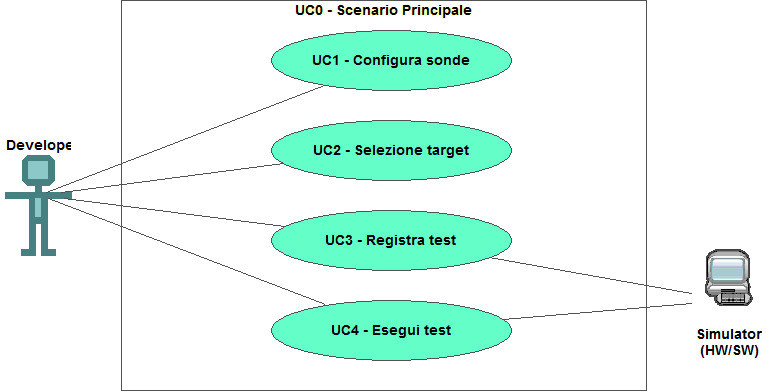
\includegraphics[width=0.75\columnwidth]{img/usecase/scenario-principale.jpeg} 
    \caption{Use Case 0: Scenario principale}
    \label{fig:scenario_principale}
\end{figure}

\begin{usecase}{0}{Scenario principale}
    \usecaseactors{Sviluppatore applicativi.}
    \usecasepre{Lo sviluppatore è entrato nel plugin di simulazione all'interno dell'IDE.}
    \usecasedesc{La finestra di simulazione mette a disposizione i comandi per configurare, registrare o eseguire un test.}
    \usecasepost{Il sistema è pronto per permettere una nuova interazione.}
    \label{uc:uc_scenario_principale}
\end{usecase}

\begin{usecase}{1}{Gestione Utente}
    \usecaseactors{Amministratore, Utente Registrato.}
    \usecasepre{L'utente deve essere autenticato nel sistema.}
    \usecasedesc{L'utente può gestire le informazioni del proprio profilo.}
    \usecasepost{Le modifiche vengono salvate nel sistema.}
    \usecasealt{Se l'utente non è autenticato, visualizza un messaggio di errore.}
    \label{uc:uc_casi_uso}
\end{usecase}

\begin{usecase}{2}{Creazione Prodotto}
    \usecaseactors{Amministratore.}
    \usecasepre{L'amministratore ha effettuato l'accesso al sistema.}
    \usecasedesc{L'amministratore può aggiungere un nuovo prodotto al catalogo.}
    \usecasepost{Il nuovo prodotto viene aggiunto con successo.}
    \usecasealt{Se i campi obbligatori non sono compilati, visualizza un messaggio di errore.}
    \label{uc:uc_creazione_prodotto}
\end{usecase}

\section{Tracciamento dei requisiti}
Da un'attenta analisi dei requisiti e degli use case effettuata sul progetto è stata stilata la tabella che traccia i requisiti in rapporto agli use case.\\
Sono stati individuati diversi tipi di requisiti e si è quindi fatto utilizzo di un codice identificativo per distinguerli.\\
Il codice dei requisiti, dove ogni requisito è identificato con il carattere \textbf{R}, è così strutturato:
\begin{enumerate}
    \item[\textbf{F}:] Funzionale.
    \item[\textbf{Q}:] Qualitativo.
    \item[\textbf{V}:] Di vincolo.
    \item[\textbf{N}:] Obbligatorio (necessario).
    \item[\textbf{D}:] Desiderabile.
    \item[\textbf{Z}:] Opzionale.
\end{enumerate}

Nelle tabelle \ref{tab:requisiti_funzionali}, \ref{tab:requisiti_qualitativi} e \ref{tab:requisiti_vincolo} sono riassunti i requisiti e il loro tracciamento con gli use case delineati in fase di analisi.

\section{Tabelle dei requisiti}
\begin{center}
    \begin{longtable}{|p{2.25cm}|p{7.75cm}|p{2.25cm}|}
    \hline \multicolumn{1}{|c|}{\textbf{Requisito}} & \multicolumn{1}{c|}{\textbf{Descrizione}} & \multicolumn{1}{c|}{\textbf{Use Case}} \\ \hline 
    \endfirsthead
    
    \multicolumn{3}{c}%
    {{\bfseries \tablename\ \thetable{} -- Continuo della tabella}} \\
    \hline \multicolumn{1}{|c|}{\textbf{Requisito}} & \multicolumn{1}{c|}{\textbf{Descrizione}} & \multicolumn{1}{c|}{\textbf{Use Case}} \\ \hline 
    \endhead
    
    \hline \multicolumn{3}{|r|}{{Continua nella prossima pagina...}} \\ \hline
    \endfoot
    \endlastfoot
    
    RFN-1 & L'interfaccia permette di configurare il tipo di sonde del test & UC1 \\
    \hline
    
    \caption{Tabella del tracciamento dei requisiti funzionali.}
    \label{tab:requisiti_funzionali}
    \end{longtable}
\end{center}

\begin{center}
    \begin{longtable}{|p{2.25cm}|p{7.75cm}|p{2.25cm}|}
    \hline \multicolumn{1}{|c|}{\textbf{Requisito}} & \multicolumn{1}{c|}{\textbf{Descrizione}} & \multicolumn{1}{c|}{\textbf{Use Case}} \\ \hline 
    \endfirsthead
    
    \multicolumn{3}{c}%
    {{\bfseries \tablename\ \thetable{} -- Continuo della tabella}} \\
    \hline \multicolumn{1}{|c|}{\textbf{Requisito}} & \multicolumn{1}{c|}{\textbf{Descrizione}} & \multicolumn{1}{c|}{\textbf{Use Case}} \\ \hline 
    \endhead
    
    \hline \multicolumn{3}{|r|}{{Continua nella prossima pagina...}} \\ \hline
    \endfoot
    \endlastfoot
    
    RQD-1n & Le prestazioni del simulatore hardware deve garantire la giusta esecuzione dei test e non la generazione di falsi negativi & - \\
    \hline
    \caption{Tabella del tracciamento dei requisiti qualitativi.}
    \label{tab:requisiti_qualitativi}
    \end{longtable}
\end{center}

\begin{center}
    \begin{longtable}{|p{2.25cm}|p{7.75cm}|p{2.25cm}|}
    \hline \multicolumn{1}{|c|}{\textbf{Requisito}} & \multicolumn{1}{c|}{\textbf{Descrizione}} & \multicolumn{1}{c|}{\textbf{Use Case}} \\ \hline 
    \endfirsthead
    
    \multicolumn{3}{c}%
    {{\bfseries \tablename\ \thetable{} -- Continuo della tabella}} \\
    \hline \multicolumn{1}{|c|}{\textbf{Requisito}} & \multicolumn{1}{c|}{\textbf{Descrizione}} & \multicolumn{1}{c|}{\textbf{Use Case}} \\ \hline 
    \endhead
    
    \hline \multicolumn{3}{|r|}{{Continua nella prossima pagina}} \\ \hline
    \endfoot
    \endlastfoot
    
    RVO-1 & La libreria per l'esecuzione dei test automatici deve essere riutilizzabile & - \\
    \hline
    \caption{Tabella del tracciamento dei requisiti di vincolo.}
    \label{tab:requisiti_vincolo}
    \end{longtable}
\end{center}

\newpage